\documentclass[11pt]{article}

% Packages
\usepackage{amsmath}
\usepackage{graphicx}
\usepackage{amssymb}
\usepackage{longtable}
\usepackage[spanish]{babel}
\usepackage[utf8]{inputenc}
\usepackage[T1]{fontenc}
\usepackage{float}


\author{Brian Ameht Inclán Quesada C-411\\ Davier Sánchez Bello C-412\\ Eric López Tornas C-411}
\title{Proyecto Final de IA y Simulación \\ Juego de Supervivencia}
\date{}

% Document
\begin{document}

\maketitle
\newpage

\tableofcontents
\newpage

\section{Introducción}
SugarScapes, expuesto extensamente en el libro "Growing Artificial Societies", publicado en 1996 bajo la autoría de Joshua Epstein y Robert Axtell, es un modelo de simulación clásico que, a través de una simulación bastante simple, con agentes de un comportamiento muy sencillo y pocos rasgos a modelar, logra simular con resultados muy realistas los comportamientos de las sociedades humanas en cuanto a distribución de la riqueza, transmisión cultural, reproducción, combates, entre otros.
En SugarScapes, los agentes carecen de una verdadera IA detrás de sí, y son más bien homogéneos a pesar de sus diferentes rasgos, debido a que todos actúan de manera similar en la mayor parte de las simulaciones inspiradas en SugarScapes.
Nosotros, quisimos explorar el tema de la violencia y la formación de agrupaciones (bandas de gángster y demás) en la sociedad, a través de nuestra propia versión de SugarScapes, pero cargando a los agentes de un comportamiento basado en IA. Queremos estudiar cuánto influyen el rango de visión, de movimiento, la riqueza heredada por un agente, su nivel de consumo, así como la zona en que nacen en su supervivencia en un ambiente donde la repartición de los recursos naturales que aparecen distribuidos de manera desigual está signada por la ley del más fuerte, por la violencia. Así, algunos agentes elegirán asociarse a otros, bajo ciertas reglas de asociación, mientras otros elegirán huir de los conflictos todo el tiempo y otros provocarlo. ¿Cuál de estas estrategias es mejor, es mejor la misma para cada tipo de agente en cuando a su capacidad de visión, movimiento y herencia, o para cada nivel de capacidad hay una estrategia que más probablemente le asegure la supervivencia? Estas y otras preguntas que nos plantearemos son fácilmente extrapolables, al igual que nuestra simulación, a situaciones de la vida real, donde los individuos deben agruparse para tener más fuerza y/o ejercerla sobre los demás, para sobrevivir, o incluso alcanzar más poder.
\section{Modelo}
\subsection{Resumen del modelo}
Emparentado a SugarScapes, nuestro modelo consiste en una grilla bidimensional, donde conviven diferentes tipos de agentes. Cada agente ocupa una casilla de la grilla, y cada casilla puede soportar una cantidad máxima de azúcar, que varía para cada una. Todos los turnos las casillas que no han alcanzado su máximo potencial de azúcar, incrementan en 1, aunque este parámetro es ajustable, la cantidad de azúcar que contienen. Cada vez que los agentes visitan una casilla, recogen todo el azúcar presente en esta, e incrementan sus reservas en la cantidad de azúcar recogida. Deben, todos los turnos, satisfacer su necesidad diaria de azúcar, consumiendo sus propias reservas. Si en algún momento sus reservas caen de 0, mueren.
Los agentes podrán interactuar entre sí atacándose o haciendo asociaciones. Una asociación es un pacto entre dos o más agentes donde cada uno acuerda ceder un determinado porcentaje de sus ganancias a la asociación y luego a cada cual le corresponde una porción de las ganancias totales de la asociación. Podrían además implementarse otras formas de relaciones sociales como las extorsiones.
Los agentes tendrán diferentes rangos y formas de movimientos, de visión y de ataques, así como nacerán con diferentes necesidades de consumo y reservas.
\subsection{Ventajas}
La principal ventaja de este modelo de simulación es que incluso tras introducir IA a los agentes y complejizar sus relaciones, la simulación sigue siendo lo suficientemente simple como para incorporar un volumen considerable de agentes, de diferentes tipos, y correr un volumen suficiente de simulaciones como para llegar a conclusiones. Otra ventaja de este modelo es que, estando basado en la experiencia previa del SugarScapes, sabemos y podemos comprobar que emula muy bien los fenómenos ocurridos en la tan compleja sociedad humana, partiendo de una simulación muy sencilla.
\subsection{Desventajas}
La principal desventaja que encontramos en este modelo para estudiar las agrupaciones de violencia en las sociedades humanas es que no toma en cuenta la compatibilidad de carácter entre los agentes, o sea, todos los agentes pueden tener el mismo tipo de relaciones con todos los demás agentes. En la vida real, el carácter de algunas personas les hace más difícil e incluso imposible mantener algún tipo de relación con otras personas, mientras que facilita el acercamiento entre otras. El modelo descrito realmente no toma en cuenta esta arista tan importante del factor humano.
\subsection{Posibles mejoras}
Respecto a la desventaja presentada anteriormente, se podrían evaluar para incrementar en cuanto a realismo la simulación, ciertas soluciones propuestas precisamente en el libro "Growing Artificial Societies". En tal libro, se logra modelar características culturales de los individuos como cadenas de bits donde ciertas propiedades de la cadena, ya fuera la posición de los bits encendidos y apagados o la cantidad total de tales bits, sirven para agrupar a los agentes en diferentes categorizaciones, y sirven como su diferenciador cultural. Muy bien podríamos emplear esta variante para simular el carácter de los agentes y determinar cuáles tienen relaciones más fluidas con otros, lo cual pudiera ser un factor para retrasar sus comunicaciones, o que influya en sus tomas de decisiones.
Otra mejora que se podría hacer a la simulación, y que parece obvia dado el tema escogido, es la introducción de relaciones familiares entre los agentes, de manera que, al avanzar la simulación, los clanes terminarían nucleando a una o unas pocas familias cada uno, y las relaciones familiares se convirtieran en un medio de poder, tal y como sucede en las agrupaciones mafiosas y las bandas violentas que intentamos emular.

\section{Implementación}
\subsection{Modelo de la simulación}
La simulación fue implementada de la manera más escalable posible. Por tal motivo, tenemos una interfaz ISimulation, que abstrae los métodos relativos a una simulación que pueden ser modificados de una simulación a otra, digase la forma de resolver los ataques o las propuestas de asociaciones. Comencemos hablando entonces de esta interfaz ISimulation y sus métodos no abstractos.
La simulación es episódica, y simulamos cada episodio usando el método step. Cada episodio es una ejecución de step. Fijamos la forma en que ocurre cada episodio, y es de la siguiente manera:
-Primeramente actualizamos a cada agente acerca de lo que puede ver, con la invocación del método $\_\_actualize_agents_vision\_\_$.
-Luego recogemos las propuestas de asociación que cada agente desea realizar, usando el método $\_\_get_association_proposals\_\_$; así como los ataques que cada agente desea realizar, usando el método $\_\_get_attacks\_\_$.
-Posteriormente son ejecutadas las propuestas de asociación y los ataques en ese orden con los métodos declarados abstractos que fueron mencionados anteriormente.
-Luego se recogen las intenciones de movimiento de cada agente, con $\_\_get_moves\_\_$, y se ejecutan con $\_\_execute_moves\_\_$.
-Luego cada agente incrementa sus reservas acorde a la cantidad cosechada en la casilla en que se encuentra y más tarde consume la cantidad que debe consumir. Los agentes cuyas reservas alcanzan números negativos, señal de que no les alcanzó para satisfacer sus necesidades, son retirados de la simulación.
-Finalmente, cada casilla que no haya alcanzado la cantidad de azúcar acumulada máxima, incrementa en 1 su cantidad de recursos.
Ahora vayamos a fondo y veamos de qué manera funciona cada uno de estos métodos, así como la descripción de los tipos usados en la simulación.
Toda simulación cuenta con un Map, y con un diccionario llamado agents que para cada ID de agente le hace corresponder un $Agent\_Handler$.
El mapa de una simulación almacena tres tipos de información: la información relativa a la presencia de agentes y objetos en las diferentes posiciones, la información relativa a la cantidad de azúcar en cada posición y la información relativa a las acciones que han sido ejecutadas desde una determinada posición en el turno anterior. Dado que asumimos que en toda casilla puede haber solo un agente o solo un objeto, y todo objeto o agente de la simulación tiene un ID único, entonces dada la biyección entre las posiciones del tablero y aquello que almacenan, manejamos las posiciones de agentes y objetos usando un bidict, estructura de Python para tuplas donde se puede hacer un lookup en O(1) tanto por llave como por valor. La información de la cantidad de azúcar en cada casilla, la cantidad máxima de azúcar en cada casilla y las acciones ocurridas en el último turno, son manejadas usando diccionarios comunes de Python
El mapa presenta métodos para insertar o mover objetos o agentes, insertar acciones, eliminar agentes o objetos en una posición específica o con un ID específico, así como averiguar la posición de un agente u objeto con un ID específico, o averiguar el contenido de una casilla en específico. Además, el mapa tiene métodos para aumentar en 1 la cantidad de azúcar que tiene cada casilla no llena y para que cada agente coseche la cantidad de azúcar que le corresponde debido a la casilla en que se encuentra.
Las acciones son almacenadas en el mapa como una lista por cada posición con las acciones tomadas desde esa posición en el turno anterior. Tales acciones son representadas por instancias de la clase Action o de la clase $Action\_Info$, o alguno de los tipos que heredan de ellos. Ambas jerarquías de tipo se usan para guardar para su transformación información relativa a los eventos de la simulación, y se usan, al menos en el caso de su presencia dentro de Map, para informar al agente acerca de lo que ha ocurrido a su alrededor.
Las simulaciones cuentan además, como habíamos mencionado anteriormente, con un diccionario que para cada ID de agente le hace corresponder un $Agent\_Handler$. $Agent\_Handler$ es la clase encargada de manejar toda la información relativa a un agente de la simulación, establecer comunicación con él, informándole de todo aquello que puede ver, las acciones que lo afectan y además preguntándole qué acciones desea realizar y verificando si tales acciones son válidas. Dentro de la información que guarda $Agent\_Handler$ encontramos, por ejemplo, las asociaciones a las que pertenece, quiénes son sus aliados, su nivel de azúcar, el porcentaje de sus ganancias que no ha comprometido aún con ninguna organización, su consumo diario, etc.
La capacidad de movimiento de un agente, su rango de visión y de ataque, están dados por instancias de las interfaces IMovement, IVision, IAttack\_Range, y tanto el $Agent\_Handler$ como el propio agente son informados de sus capacidades, de manera que el $Agent\_Handler$ puede descartar cualquier acción del agente que no sea válida, así como el agente está en condiciones de deducir qué acciones puede tomar.
Los agentes cumplen con la interfaz IAgent que plantea la API a través de la cual los agentes se comunican. Esta API tiene dos clases de métodos: los informativos que pasan al agente datos sobre la simulación, digase aquello que pueden ver, o las acciones que los afectan directamente, y métodos para obtener las acciones que el usuario desea realizar en cada episodio de la simulación.
Además, nuestros agentes todos heredan de $Agent\_With\_Memory$. $Agent\_With\_Memory$ mantiene guardada toda la información que un agente puede necesitar para la toma de sus decisiones. Guarda toda la información proveniente de las visiones del agente en 4 tipos de memorias diferentes: la memoria para visiones de agentes, la memoria geográfica, la memoria para los ataques y la memoria para las asociaciones. Estas memorias están diseñadas de manera que se pueda realizar eficientemente cualquier tipo de query acerca de lo que un agente ha visto, proporcionando escalabilidad, por si es necesario para alguna nueva IA información que anteriormente no habíamos pensado que importara. Para lograr esa eficiencia, las memorias guardan la información que le corresponde a cada una en tablas de SQLite almacenadas en memoria del programa (es decir, una base de datos no persistente).
Si bien en la simulación, las casillas tienen un sistema de posicionamiento absoluto, donde la casilla en el extremo superior izquierdo es la (0, 0) y aumentan a partir de ahí, quisimos, para hacer la simulación más cercana a un combate en un terreno desconocido, como sucede en Los Juegos del Hambre, nuestra inspiración inicial para el proyecto, que los agentes no conozcan la posición absoluta de cada casilla dentro del tablero. Siendo así, todo cuanto los agentes ven les es comunicado en posición relativa, respecto a donde se encuentran, tal como en la vida real, vemos que algo se encuentra aproximadamente a tres pasos de distancia y no las coordenadas exactas donde se encuentra
O sea, la comunicación entre el agente y el mundo de la simulación ocurre en términos de posiciones relativas respecto a la posición del agente. Es decir, cuando el agente dice que desea moverse a una determinada posición, comunica que se desea mover a la posición que se encuentra, por ejemplo, tres filas más arriba y dos columnas a la derecha de donde se encuentra ahora mismo, y de manera idéntica, cuando le comunican la presencia de un objeto, esto ocurre a través de posiciones relativas respecto a la posición del agente
No obstante, el agente para recordar con precisión debe tener para sí un sistema de coordenadas absolutas. Esto lo modelamos centrando sus coordenadas en la casilla en la cual el agente comienza la simulación, llamándola (0, 0), y manteniendo todo el tiempo en qué posición se encuentra el agente con respecto a dónde comenzó. Así también es posible conocer en qué posición respecto al (0, 0) se encuentra cada objeto o agente o montón de azúcar visto por el agente. Todo este aspecto de mantener la posición del agente dentro de su propio sistema de coordenadas y asignarle posición a cada uno de los objetos lo manejamos dentro de $Agent\_with\_Memories$, de manera que no es una preocupación a la hora de implementar ninguno de los agentes que heredan de él.
Enumeremos brevemente las memorias de un agente y sus features.
La $Memory\_for\_Agents_Sights$ mantiene un conjunto con los ID de todos los agentes que el agente propietario de la memoria ha visto, y que no ha visto morir aún. Mantiene además, una tabla donde para cada agente hay una entrada con el número de iteración en que ocurrió la observación, el ID del agente observado, la posición donde fue observado y la cantidad de azúcar que llevaba consigo. Luego, $Memory\_for\_Agents\_Sight$ tiene una serie de métodos que permiten consultar esta tabla para averiguar ya sea donde el agente vio por última vez a un determinado agente, o qué contenido tenía determinada posición en un turno determinado; hasta la historia completa de las observaciones de algún agente. Todos estos métodos son muy útiles a la hora de tomar decisiones, ya que ayudan a medir con mayor o menor exactitud dónde se encuentra cada uno de los otros agentes.
La $Geographic\_Memory$ mantiene un conjunto con todas las posiciones que el agente ha visto a lo largo de la simulación. Ya que, tal como mencionamos, el agente no conoce de antemano el medio donde se encuentra ni sus límites, solamente puede conocer si una posición es válida (se encuentra dentro de la simulación) si la ha visto de antemano. Además, $Geographic\_Memory$ se encarga de almacenar la información concerniente a la cantidad de azúcar vista en cada posición por el agente. Tiene para cada casilla la cantidad de azúcar que el agente vio la última vez que pudo observar esa casilla, junto al dato de cuándo ocurrió tal observación, además de para cada casilla cuál es la máxima cantidad de azúcar observada por el agente en tal posición. Ambos datos son importantes para el agente realizar sus cálculos acerca de a dónde moverse para recolectar la mayor cantidad de azúcar posible.
La $Memory\_for\_Attacks$ mantiene los datos acerca de todos los ataques que el agente ha presenciado en otra tabla de SQLite, de manera que se puede hacer cualquier clase de consultas acerca de qué ataques ha realizado o recibido algún agente, con cuánta fuerza, cuándo fue la última vez que lo hizo y demás. Algunos consultas que percibimos serían más frecuentes y útiles para nuestro propio uso tienen sus propios métodos, pero se pueden añadir nuevos métodos para nuevas consultas a medida que sean necesarias. La información brindada por esta tabla ayuda a determinar el carácter de cada uno de los demás agentes así como a estimar más o menos cuántos recursos deberían quedarle. La $Memory\_for\_Attacks$ tiene además una lista con todos los agentes que han fallecido en la simulación, ya sea por causas naturales o por ataques realizados en su contra.
La $Memory\_for\_Associations$ mantiene para cada asociación cuya creación el agente ha presenciado el turno en que fue creada. Si el agente pudo precisar los datos de cada asociación al ser creada, digamos sus miembros y los compromisos de cada uno de ellos, entonces esos datos son mantenidos en una tabla de SQLite donde cada entrada corresponde al compromiso de un agente en una asociación específica. Luego, es posible realizar todo tipo de consultas acerca de a qué asociaciones pertenece un agente determinado, o cuáles son sus compromisos, o quiénes son los agentes que presentan compromisos más elevados, en fin..., cualquier consulta que pueda brindar información valiosa para la toma de decisiones del agente y que este relacionada a datos sobre asociaciones.
Además, un $Agent\_with\_Memories$ mantiene otras informaciones que no llegan precisamente a través de la visión del agente, sino a través de métodos de la API de IAgent destinados a informar al agente de acciones que lo afectan directamente como su incorporación o salida de asociaciones o la culminación exitosa de un ataque hecho por el mismo o recibido, o que se culminó su movimiento a otra posición. Se guardan de esta manera las posiciones donde el agente ha estado, los movimientos que ha hecho, los ataques que ha realizado o que ha recibido. Además, $Agent\_with\_Memories$ mantiene el dato acerca de las reservas de azúcar que tiene el agente.
En definitiva, $Agent_With_Memories$ es una clase abstracta que implementa algunos de los métodos de IAgent para mantener almacenada toda la información que las diferentes implementaciones de agentes pueden necesitar a lo largo de la simulación para sus procesos de toma de decisiones.
Nos queda por hablar de algunos métodos de ISimulation, antes de pasar a la implementación puntual de esta interfaz que usamos en el proyecto.
El método $\_\_execute\_moves\_\_$ pasa todos los movimientos al mapa y deja a este encargarse de manejarlos. Con la implementación de Map que usamos, si dos agentes coinciden en cuanto a la casilla a la que desean moverse, no se mueven en lo absoluto, tal y como si decidieran moverse a posiciones no válidas.
El método $\_\_get\_association\_proposals\_\_$ toma las propuestas de asociación que realiza cada agente y comprueba su validez con otro método de ISimulation, $\_\_validate\_association\_proposals\_\_$.
Las asociaciones tienen por ID al hash de la tupla formada por el ID de sus miembros en orden, de manera que no será posible que el mismo conjunto de agentes tenga más de una asociación que los una. Para verificar que se cumpla tal ley, sencillamente basta con no aceptar propuestas de asociaciones que generarían una asociación con un ID ya existente. Además, se verifica que todos los miembros de la asociación propuesta estén vivos y puedan cumplir con el porcentaje de sus ganancias que deben entregar acorde a sus compromisos. Además, se comprueba que todos los valores de los compromisos sean correctos.
A diferencia del $get\_association\_proposals$, en $\_\_get\_attacks\_\_$ la validación de los ataques solicitados por el agente es delegada al $Agent\_Handler$ que mantiene comunicación con el agente, pues es este quien posee toda la información relativa al agente y pueda verdaderamente discernir si un ataque es válido o no.
El método $\_\_feed\_single\_agent\_\_$ se encarga de entregar a un agente las reservas que le corresponden debido a una ganancia en particular, ya sea por una cosecha realizada o por haber matado a algún agente. En caso de que el agente esté asociado, delega en el método feed de cada instancia de asociación a la que el agente pertenece la responsabilidad de repartir a cada agente de la asociación cuánto le corresponde ganar por este evento en particular. El agente toma luego aquella porción de la ganancia que aún no ha comprometido con ninguna asociación. Cada agente es informado además del motivo de la ganancia, si fue un asesinato o una cosecha normal, debido a que el método a través del cual le es informada la ganancia le provee de tal información.
El método $\_\_feed\_agents\_\_$ entrega a cada agente las cosechas que le corresponden de la posición en que se encuentra, haciendo uso del método $\_\_feed\_single\_agent\_\_$ para manejar cada caso particular. Además, este método llama a $\_\_remove\_agent\_\_$ para sacar de la simulación a todos aquellos agentes cuyas reservas hayan caído en números negativos.
El método $\_\_remove\_agent\_\_$ como su nombre indica saca a un agente de la simulación y, si estaba asociado, disuelve la asociación en la que se encontraba haciendo uso del método $\_\_remove\_association\_\_$.
El método $\_\_remove\_association\_\_$ informa a cada agente involucrado en la asociación destruida de la destrucción de esta a través de un método de $agent\_handler$ que conecta con un método de IAgent del mismo nombre, $inform\_broken\_association$. Los agentes ajenos a la asociación pero que tienen a algunos de sus miembros en su rango visual se enteran de la disolución de la asociación porque una acción $Association\_Destruction$ es colocada en el mapa en la posición de cada uno de los agentes pertenecientes a la asociación, y luego tal acción llega al conocimiento de los agentes a través de su visión.
Respecto a la implementación puntual que tenemos de la simulación, comencemos exponiendo cómo se manejan los ataques.
En $simple\_simulation$, la simulación que hicimos, los ataques cuestan a los agentes que los realizan, mientras más invierten en el ataque más daño causa este en el rival. Dada la naturaleza simple de la simulación, no modelamos el combate de una manera compleja, asumimos que los ataques siempre llegan a su destino y producen el mismo daño no importa la circunstancia. No obstante, en la propia $Simple\_Simulation$ dejamos la puerta abierta a cualquier tipo de simulación de ataques de mucho más complejidad que será descrito a continuación.
Primeramente, recogemos los ataques que desea realizar cada agente, de manera que los ejecutemos de manera simultánea. Luego, instanciamos un grafo con tales ataques y nos quedamos con sus componentes conexas. Cada componente conexa es un combate, y tiene sentido procesar cada componente conexa, porque, en una situación de combate real, si muchos atacan a la misma vez a un agente, por ejemplo, pueden potenciar el daño de sus ataques al no poder este esquivarlos, o si un agente es atacado, la fuerza de los ataques que realiza en ese instante se ve debilitada. O sea, podríamos, de haber querido, complejizar la simulación de la batalla tanto como hubiéramos querido, dada la expresividad que tiene la modelación de los combates como grafos.
Por su parte, en el método $\_\_execute\_associations\_proposals\_\_$, preguntamos a cada agente si desea formar parte de la asociación que se propone. En caso de que todos los potenciales miembros acepten, les informamos a cada uno acerca de su nueva afiliación y añadimos al mapa una acción de tipo $Association\_Creation$ con los datos de la asociación creada en cada posición de agente unido a la asociación. De manera que aquellos cercanos geográficamente a él puedan conocer acerca de la ocurrencia de la asociación y sus detalles.
Implementamos unos pocos rangos simples para hacer funcionar a los agentes, digamos, caminar un solo paso en las direcciones principales en SimpleWalking o atacar y observar cualquier objeto en un cuadrado de radio provisto a su alrededor en SquareVision y $SquareRange\_of\_Attack$. Pero crear otros tipos de rangos de visión, ataque o movimiento no supone una dificultad, tan solo habría que heredar de las interfaces correspondientes.
\subsection{Agentes}
En nuestra simulación de supervivencia, utilizamos varios tipos de agentes, cada uno con estrategias y objetivos específicos que influyen en su comportamiento dentro del juego.Todos tienen un sistema experto que emula el conocimiento y la toma de decisiones del agente,
basandoce en la información que se le proporciona en el entorno de juego. Estas desiciones se toman en dependencia de las regls que se definan en el sistema experto, más explicado adelante. A continuación, describimos los tipos de agentes que utilizamos en nuestra simulación:

\subsubsection{Agente Aleatorio (RandomAgent)}
El \textit{RandomAgent} es un tipo de agente diseñado para tomar decisiones de manera aleatoria dentro de un entorno simulado. Este agente es una extensión de \textit{Agent\_with\_Memories}, lo que implica que puede recordar interacciones pasadas y datos del entorno para influir en sus decisiones futuras. Utiliza un sistema de estrategia basado en hechos y reglas para manejar su comportamiento en la simulación.

\paragraph{Funcionalidad del \textit{RandomAgent}}
\begin{itemize}
    \item \textbf{Inicialización}: Al crearse, se le asignan varios hechos iniciales como alianzas, enemigos, movimientos posibles, y recursos, entre otros. Estos hechos forman la base de su toma de decisiones.
    \item \textbf{Movimiento}: El agente decide su próximo movimiento de forma aleatoria entre los movimientos posibles disponibles, basándose en la estrategia actual.
    \item \textbf{Ataque}: Puede decidir atacar a otros agentes en su entorno si los ve. La decisión de atacar y la selección del objetivo son aleatorias, y el ataque se divide equitativamente entre los agentes visibles.
    \item \textbf{Asociaciones}: El agente puede recibir propuestas para unirse a asociaciones y decide aleatoriamente si unirse o no.
    \item \textbf{Interacción con el entorno}: Recibe y procesa información sobre objetos, recursos y acciones de otros agentes dentro de su entorno.
\end{itemize}

\paragraph{Reglas Definidas}
\begin{enumerate}
    \item \textbf{Regla de Movimiento (\textit{move\_rule})}:
          \begin{itemize}
              \item \textbf{Condición}: Se activa si hay movimientos posibles disponibles.
              \item \textbf{Acción}: Elige un movimiento aleatoriamente de los posibles y lo establece como el próximo movimiento.
          \end{itemize}
    \item \textbf{Regla de Ataque (\textit{attack\_rule})}:
          \begin{itemize}
              \item \textbf{Condición}: Se activa si hay otros agentes visibles en el entorno y decide aleatoriamente si realizar un ataque.
              \item \textbf{Acción}: Si decide atacar, distribuye los recursos de ataque disponibles equitativamente entre los agentes visibles y selecciona un subconjunto aleatorio de estos para atacar.
          \end{itemize}
\end{enumerate}

Estas reglas permiten al \textit{RandomAgent} operar en un entorno dinámico donde las decisiones no siguen un patrón predecible, lo que puede ser útil para simular comportamientos impredecibles o para probar la robustez de otros agentes dentro de la simulación.

\subsubsection{Agente Pacífico (PacifistAgent)}
El \textit{PacifistAgent} es un agente diseñado para evitar conflictos y minimizar las interacciones hostiles dentro de la simulación del juego de supervivencia. Este agente sigue una estrategia de no agresión, priorizando la evasión y la preservación por encima de la confrontación. A continuación, se describen sus funcionalidades y las reglas específicas que guían su comportamiento en el entorno simulado.

\paragraph{Funcionalidades del \textit{PacifistAgent}}
\begin{itemize}
    \item \textbf{Inicialización}: Al inicio, el agente configura hechos iniciales como alianzas, enemigos, y otros agentes en el entorno. Establece su memoria geográfica y de ataques, lo cual influye en su toma de decisiones estratégica.
    \item \textbf{Decisiones de Movimiento}: Basa sus movimientos en un conjunto de reglas evaluadas continuamente para elegir rutas que maximicen la distancia de las amenazas.
    \item \textbf{Reacción a Ataques}: Actualiza su conocimiento sobre enemigos y modifica su ruta al recibir ataques para mantenerse lo más distante posible del atacante.
    \item \textbf{Interacción Social}: Puede recibir propuestas de asociación y decide si participar basándose en su estrategia de no confrontación.
    \item \textbf{Observación del Entorno}: Continuamente actualiza su base de conocimientos con información sobre objetos y acciones observadas para tomar decisiones informadas.
\end{itemize}

\paragraph{Reglas del \textit{PacifistAgent}}
\begin{enumerate}
    \item \textbf{Regla para Moverse Lejos del Atacante (\textit{move\_away\_rule})}:
          \begin{itemize}
              \item \textbf{Condición}: Activada al recibir un ataque.
              \item \textbf{Acción}: Calcula y ejecuta un movimiento que incrementa la distancia entre él y el atacante.
          \end{itemize}
    \item \textbf{Regla para Observar Objetos (\textit{see\_objects\_rule})}:
          \begin{itemize}
              \item \textbf{Condición}: Activada cuando hay objetos visibles que pueden representar una amenaza.
              \item \textbf{Acción}: Evalúa y ajusta la ruta para evitar los objetos identificados como amenazas.
          \end{itemize}
    \item \textbf{Regla para Observar Acciones (\textit{see\_actions\_rule})}:
          \begin{itemize}
              \item \textbf{Condición}: Activada al observar acciones que pueden necesitar una respuesta evasiva.
              \item \textbf{Acción}: Analiza las acciones y decide la mejor ruta de evasión.
          \end{itemize}
    \item \textbf{Movimiento por Defecto (\textit{default\_move})}:
          \begin{itemize}
              \item \textbf{Condición}: Activada cuando no hay amenazas inmediatas detectadas.
              \item \textbf{Acción}: Selecciona un movimiento al azar de las opciones disponibles.
          \end{itemize}
\end{enumerate}

Estas reglas permiten al \textit{PacifistAgent} operar en un entorno dinámico y potencialmente hostil de manera que evita conflictos, lo cual es crucial para su supervivencia en el juego.

\subsubsection{Agente de Combate (CombatantAgent)}
El \textit{CombatantAgent} está diseñado para operar en entornos altamente hostiles y está enfocado en la confrontación directa. Utiliza estrategias complejas para maximizar su eficacia en el combate, respondiendo agresivamente a cualquier amenaza percibida.

\paragraph{Funcionalidades}
\begin{itemize}
    \item Inicializa con una configuración detallada de conocimientos que guiarán sus decisiones tácticas y estratégicas en el campo de batalla.
    \item Responde dinámicamente a los ataques, eligiendo la mejor acción basada en la evaluación continua del entorno.
    \item Observa y analiza constantemente el entorno para adaptar sus estrategias y movimientos.
\end{itemize}

\paragraph{Reglas Definidas}
\begin{enumerate}
    \item \textbf{Ataque a Enemigos Visibles}: Lanza ataques coordinados contra enemigos detectados dentro de su rango visual.
    \item \textbf{Movimiento Táctico}: Se mueve estratégicamente para posicionar mejor o evitar ataques.
    \item \textbf{Reacción a Ataques Recibidos}: Define la estrategia de respuesta, ya sea evasiva o de contraataque, basada en la naturaleza del ataque recibido.
    \item \textbf{Movimiento por Defecto}: Realiza un movimiento predeterminado cuando no hay decisiones claras de combate o movimiento.
\end{enumerate}

Estas reglas le permiten al \textit{CombatantAgent} manejar situaciones de combate con un enfoque estratégico y táctico, asegurando que cada acción tomada maximice su potencial de supervivencia y éxito en el combate.

\subsubsection{Agente Inteligente (SmartAgent)}
El \textit{SmartAgent} utiliza algoritmos avanzados de toma de decisiones y aprendizaje automático para adaptar su comportamiento basado en la dinámica del juego. Este agente evalúa constantemente el estado del juego, tomando decisiones informadas sobre cuándo recolectar recursos, combatir, o retirarse basado en las probabilidades de éxito y supervivencia.

\subsubsection{Agente Buscador de Comida (FoodSeekerAgent)}
El \textit{FoodSeekerAgent} es un agente programado para enfocarse intensamente en la localización y recolección de recursos alimenticios dentro de la simulación. Evita el combate en la medida de lo posible, priorizando la acumulación de recursos para garantizar su supervivencia.

\paragraph{Funcionalidades}
\begin{itemize}
    \item Configura hechos iniciales que incluyen la memoria geográfica y táctica, cruciales para la navegación y las decisiones estratégicas.
    \item Se especializa en la eficiente localización y consumo de recursos, utilizando avanzados algoritmos de búsqueda para optimizar sus rutas.
    \item Prefiere evitar conflictos, eligiendo caminos que minimicen el contacto con otros agentes agresivos.
\end{itemize}

\paragraph{Reglas Definidas}
\begin{enumerate}
    \item \textbf{Comer sin Enemigos}: Optimiza el movimiento hacia los recursos cuando no hay amenazas cercanas.
    \item \textbf{Comer con Enemigos}: Decide entre aprovechar los recursos o moverse a una posición más segura si hay enemigos cerca.
    \item \textbf{Movimiento por Defecto}: Realiza un movimiento estándar cuando no se detectan recursos o amenazas inmediatas.
    \item \textbf{Situaciones de Atasco y Recursos Disponibles}: Resuelve bloqueos en su ruta para continuar hacia los recursos.
\end{enumerate}

Estas reglas permiten al \textit{FoodSeekerAgent} operar eficazmente en un entorno donde la obtención de recursos es crucial para la supervivencia.

\subsection{Base de conocimiento y toma de decisiones}
Este sistema se basa en una estructura modular que integra hechos y reglas dentro de un motor de inferencia para gestionar y tomar decisiones basado en conocimientos. Está diseñado para funcionar en entornos donde las decisiones se toman a partir de un conjunto de datos dinámico y posiblemente en tiempo real. Los componentes clave son:

\begin{itemize}
    \item \textbf{Enumeración \textit{Knowledge}:} Es una enumeración que define diferentes tipos de conocimientos que pueden ser importantes en un contexto de toma de decisiones. Estos incluyen aspectos como la posición, la salud, los ataques disponibles, las asociaciones y más. Cada tipo de conocimiento sirve como una clave que identifica un tipo de información específica dentro del sistema
    \item \textbf{Clase \textit{Fact}:}  Representa un hecho o una pieza de información en el sistema. Cada hecho está compuesto por una clave (un valor de Knowledge) y un dato asociado a esta clave. Esta estructura permite almacenar y gestionar información dinámica que el sistema utiliza para tomar decisiones
    \item \textbf{Clase \textit{Rule}:}  Define una regla en el sistema, la cual consta de una condición y una acción. La condición es una función que toma un conjunto de hechos y determina si la regla debe ejecutarse. Si la condición es verdadera, la acción (también una función) se ejecuta para generar nuevos hechos basados en los hechos existentes. En resumen, esta clase permite definir la lógica del sistema para generar nuevos hechos a partir de los existentes.
    \item \textbf{Clase \textit{BaseKnowledge}:} Esta clase especifica las operaciones fundamentales para cualquier sistema de conocimiento, como aprender y tomar decisiones.
    \item \textbf{Clase \textit{Estrategy}:} Es una implementación concreta de BaseKnowledge. Gestiona un conjunto de hechos y reglas a través de un motor de inferencia. Permite añadir y eliminar conocimientos y reglas, aprender de nuevos datos y tomar decisiones basadas en las reglas definidas y los hechos actuales
    \item \textbf{Clase \textit{InferenceEngine}:} Es el componente que realiza la inferencia lógica. Gestiona un conjunto de hechos y reglas, permitiendo añadir y eliminar estos elementos. El método run de InferenceEngine es crucial: evalúa todas las reglas con los hechos actuales para generar nuevos hechos, los cuales pueden influir en decisiones futuras.
\end{itemize}

Este modelo permite un manejo flexible y dinámico de información, esencial para la toma de decisiones en entornos cambiantes, tal y como necesitamos en nuestra simulacion.
\subsection{Algoritmos de búsqueda}
En esta sección, describiremos varios algoritmos de búsqueda utilizados en nuestro proyecto. Cada algoritmo será tratado en una subsección independiente, donde se explicará su funcionamiento, particularidades y ejemplos de uso.

\subsubsection{Algoritmo A*}
El algoritmo A* es una técnica de búsqueda de camino que encuentra el camino más corto entre un nodo inicial y un nodo objetivo en un grafo. Utiliza una combinación de costos conocidos para llegar a un nodo \( g(n) \) y una estimación heurística \( h(n) \) del costo para alcanzar el objetivo desde ese nodo. La función \( f(n) = g(n) + h(n) \) guía el algoritmo para explorar los caminos más prometedores primero.

En nuestro caso estamos implementado usando una estructura de tipo $min-heap$, denominada $open\_heap$. Esta estructura se utiliza para mantener los nodos que aún necesitan ser explorados en el algoritmo. Mediante un heap de minimos organiza los elementos de tal manera que el primer elemento es siempre el más pequeño, lo cual es útil para extraer rápidamente el nodo con el costo estimado más bajo para continuar la búsqueda.


\paragraph{Detalles del Funcionamiento}
\begin{itemize}
    \item \textbf{Heurística}: La función heurística es crucial en A*. Una elección común es la distancia Manhattan, útil en grillas donde solo se permiten movimientos horizontales y verticales.
    \item \textbf{Conjunto de abiertos}: A* mantiene un conjunto de nodos conocidos como el "conjunto abierto". Inicialmente, contiene solo el nodo de inicio.
    \item \textbf{Bucle Principal}: En cada paso del algoritmo, el nodo con el menor valor de \( f(n) \) se retira del conjunto abierto. Este nodo es procesado considerando todos sus nodos vecinos. Para cada vecino, se calcula \( g(n) \) y \( h(n) \), y si el nuevo camino es mejor, se actualiza el camino.
\end{itemize}

\paragraph{Ejemplo de Uso}
En el siguiente ejemplo mostramos un agente del tipo $FoodSeekerAgent$ que en nuestra simulacion representa al agente que esta constantemente buscando la mejor manera de llegar al lugar donde mas recursoa halla. En este caso tenemos un tablero de \(10 \times 10\). Definimos la posición inicial como \( (0, 8) \) y el objetivo en este caso la casilla que dentro de su rango de vision
es la que mas recursos posee, como \( (2, 9) \). La salida del algoritmo proporcionará la secuencia de movimientos para llegar del inicio al objetivo, evitando los obstáculos, que en este ejemplo no hay ninguno.

\begin{figure}[H]
    \centering
    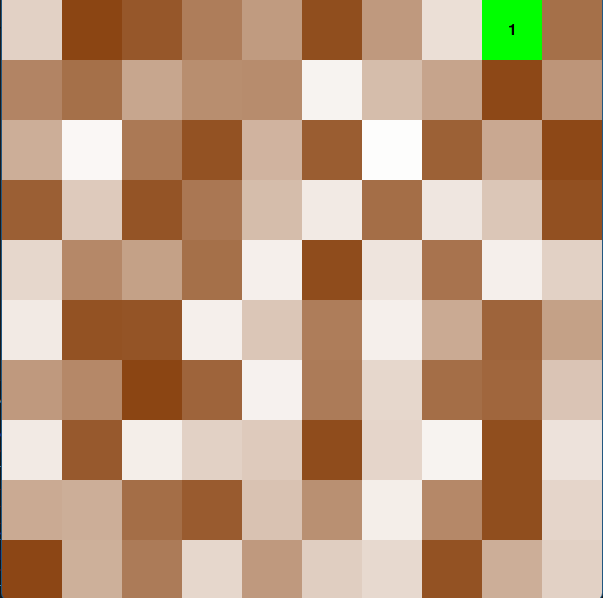
\includegraphics[width=0.18\textwidth]{images/image1.png}\hfill
    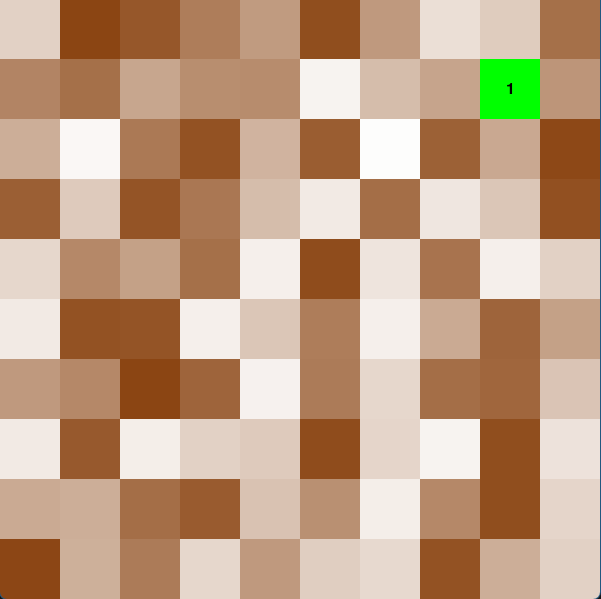
\includegraphics[width=0.18\textwidth]{images/image2.png}\hfill
    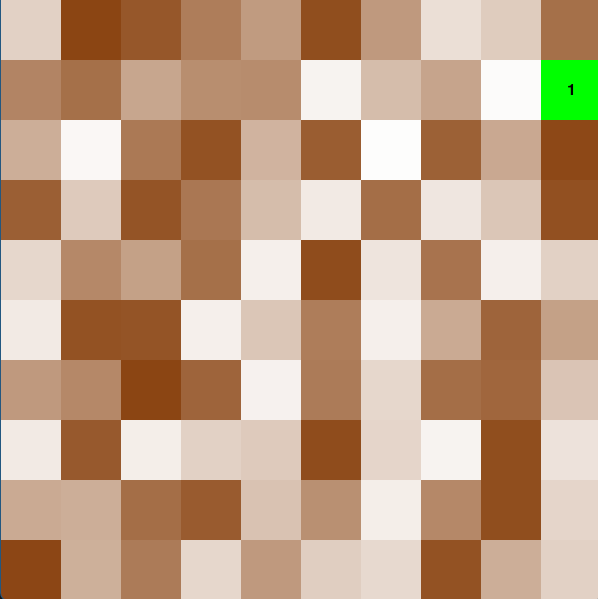
\includegraphics[width=0.18\textwidth]{images/image3.png}\hfill
    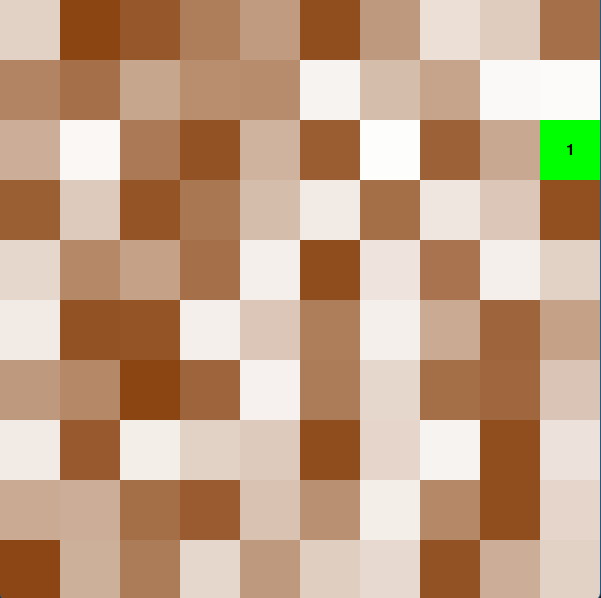
\includegraphics[width=0.18\textwidth]{images/image4.png}
    \caption{Secuencia de movimientos del agente FoodSeekerAgent en la simulación desde la posicion \( (0, 8) \) hasta \( (2, 9) \) .}
\end{figure}

\paragraph{Implementación}
Para implementar el A* en la simulación de nuestro juego, utilizamos una clase que gestiona la verificación de movimientos válidos y obstáculos. Esta clase ajusta el algoritmo para adaptarse a las características específicas del entorno de juego, como áreas inaccesibles y diferentes costos de movimiento asociados con diversos tipos de terreno.

\subsubsection{Búsqueda en Amplitud (BFS)}
La Búsqueda en Amplitud, o BFS por sus siglas en inglés (Breadth-First Search), es un algoritmo clásico para explorar grafos y árboles. Es especialmente útil en situaciones donde necesitamos encontrar el camino más corto en términos de número de aristas entre un nodo de origen y otros nodos, dado que explora todos los nodos a la misma profundidad antes de moverse a la profundidad siguiente.
En nuestra simulación está especialmente diseñado para calcular rutas de escape en situaciones donde un agente necesita maximizar la distancia de un atacante en un entorno de grilla. La adaptación permite a los usuarios elegir entre obtener sólo el siguiente movimiento óptimo o el camino completo de escape.

\paragraph{Funcionamiento de BFS}
La implementación de BFS comienza con la inserción del nodo de origen en una cola. A medida que cada nodo se procesa, sus vecinos no visitados se añaden al final de la cola. Este proceso continúa hasta que se visitan todos los nodos alcanzables o hasta que se encuentra el nodo objetivo, lo que permite una exploración completa en capas.

\begin{itemize}
    \item \textbf{Cola de BFS}: Utilizamos una cola para mantener el orden de exploración de los nodos. En nuestra implementación, esto se maneja con una estructura de datos deque para una eficiente inserción y eliminación de elementos.
    \item \textbf{Conjunto de Obstáculos y Visitados}: Mantenemos un conjunto de obstáculos para evitar la exploración de nodos no transitables y un conjunto de nodos visitados para evitar procesar el mismo nodo más de una vez.
    \item \textbf{Validación de Movimientos}: Cada movimiento potencial se valida para asegurar que no se salga del límite del entorno de juego y no se encuentre con obstáculos.
\end{itemize}

\paragraph{Ejemplo de Uso}
En el siguiente ejemplo, mostramos un agente del tipo $PacifistAgent$ \( (azul) \) en la posicion \( (5, 6) \), que en nuestra simulación representa al agente que tiene una estrategia pacifica, evade los ataques e intenta sobrevivir.
En este caso, tenemos un tablero de \(7 \times 7\). Definimos la posición inicial del agente $CombatantAgent$ \( (rojo) \) como \( (3, 3) \). La salida del algoritmo proporcionará la secuencia de movimientos para llegar a la posición segura más lejana posible, evitando al atacante, evidenciamos en las siguientes imagenes como
la secuencia de movimientos incluye como primer movimiento el de alejarce del atacante hacia la casilla \( (6, 6) \), luego en el siguiente movimiento, este se queda en esa misma posicion ya que de entre las posibles es la mas lejana al atacante


\begin{figure}[H]
    \centering
    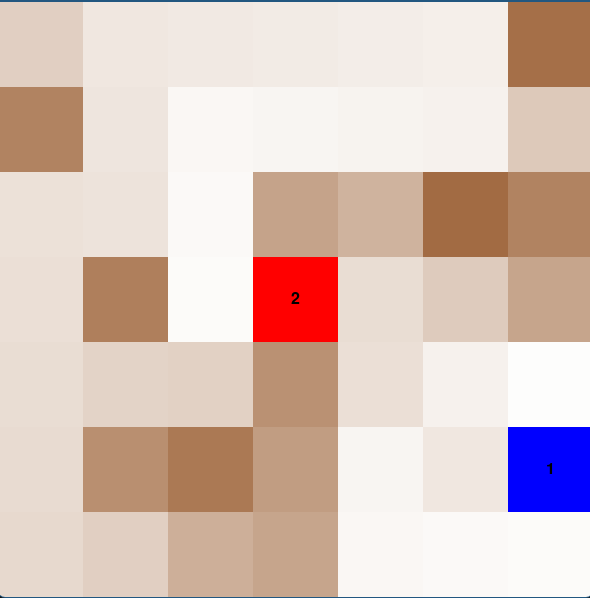
\includegraphics[width=0.18\textwidth]{images/image6.png}\hfill
    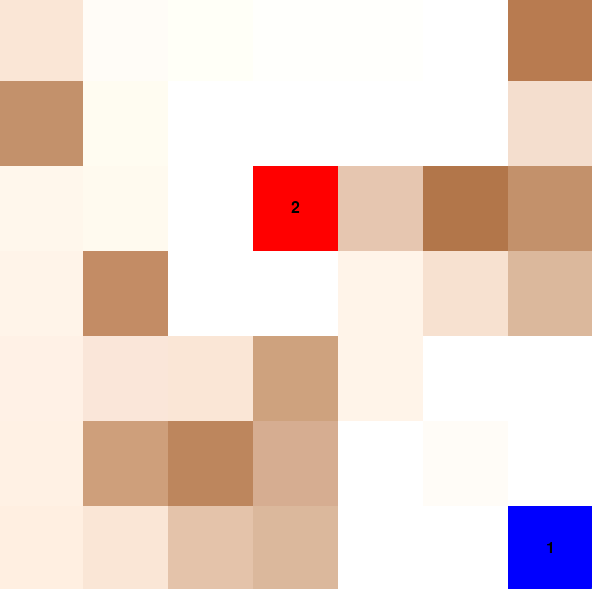
\includegraphics[width=0.18\textwidth]{images/image7.png}\hfill
    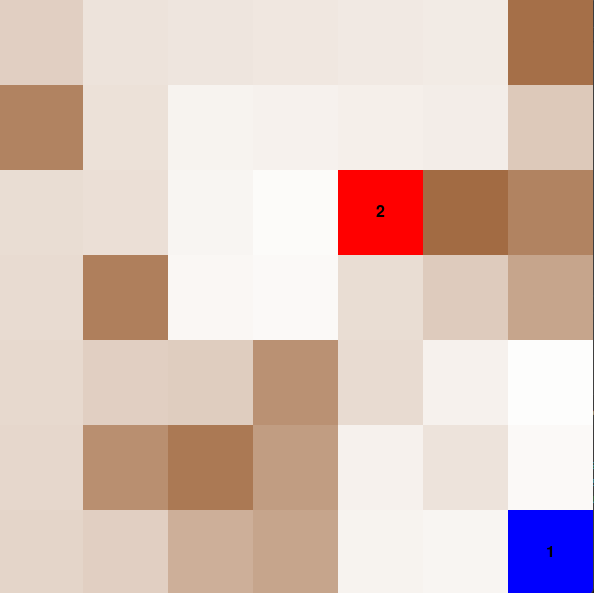
\includegraphics[width=0.18\textwidth]{images/image8.png}
    \caption{Secuencia de movimientos calculada por BFS para evadir al atacante, mostrando cada paso desde el inicio hasta la posición segura más lejana posible.}
\end{figure}

\paragraph{Implementación}
Nuestra clase \textit{BFS} incluye métodos para configurar los obstáculos y calcular la ruta basada en las posiciones dinámicas de los agentes y las barreras en el entorno. Esto asegura que el agente siempre tenga una ruta de escape actualizada y pueda reaccionar a los cambios en el entorno.



\subsubsection{Monte Carlo Tree Search (MCTS) (Trabajo en proceso)}
El Monte Carlo Tree Search (MCTS) es un algoritmo de búsqueda heurística ampliamente utilizado en la toma de decisiones en juegos y problemas de optimización combinatoria.
A diferencia de otros enfoques, como la búsqueda en profundidad, MCTS no requiere un conocimiento completo del espacio de búsqueda y es especialmente útil en entornos con una gran cantidad de acciones posibles y una complejidad elevada.\\

Este método se basa en una búsqueda inteligente de árboles que equilibra la exploración y la explotación. Utiliza el concepto de muestreo aleatorio mediante simulaciones, conocidas como "playouts", para evaluar las diferentes opciones disponibles.
A medida que se realizan más playouts, el algoritmo acumula estadísticas sobre las acciones tomadas.\\

En nuestra implementación, aplicamos MCTS para guiar al agente en la selección de acciones óptimas en un entorno simulado. Consideramos el limitado conocimiento del usuario sobre la simulación para adaptar la exploración del árbol de búsqueda
y priorizar aquellas acciones que parecen más prometedoras según las heurísticas de comportamiento implementadas en los agentes.\\

\paragraph{Funcionamiento de MCTS}
Cada vez que un agente emplea MCTS en la toma de decisiones, se crea un objeto MCTS que representa el árbol de búsqueda del agente en ese turno. La raíz de este árbol refleja el estado de la simulación justo antes de que el agente tome una decisión.
El algoritmo de MCTS sigue un ciclo de cuatro pasos:\\

\begin{itemize}
    \item \textbf{Selección}: Desde el nodo raíz R, se busca un nodo hoja L que represente un escenario de la simulación desde el cual no se ha tomado ninguna decisión.
    \item \textbf{Expansión}: A menos que el nodo L sea terminal (es decir, el agente gana o pierde), se expande el árbol de búsqueda creando uno o más nodos secundarios. Estos nodos representan movimientos válidos desde la posición de juego definida por L.
    \item \textbf{Simulación}: Se realiza una reproducción aleatoria del juego desde el nodo C, elegido durante la fase de expansión. Esta simulación proporciona una estimación del valor de ese nodo y ayuda a evaluar la calidad de las acciones disponibles.
    \item \textbf{Actualización}: El resultado de la simulación se utiliza para actualizar la información en los nodos de la ruta desde C hasta R, lo que permite al algoritmo ajustar sus estimaciones y mejorar la toma de decisiones futuras.
\end{itemize}

\paragraph{Implementación}
En nuestra implementación de MCTS, aprovechamos la información observada por el agente y su conocimiento previo de la simulación, como los agentes que ha visto cercanos o el recuento global de muertes, para construir una representación simplificada del escenario.

\paragraph{Ejemplos}
Ejemplos...



\subsection{LLM}
Utilizamos el LLM para la creación de agentes y la configuración del escenario de la simulación, así como para la función de comentarista del juego. Para la creación de agentes, empleamos una lista con descripciones por defecto de los comportamientos de nuestros tipos de personajes y la información suministrada por el usuario. El LLM infiere cuál es el tipo de personaje por defecto que más se acerca a la descripción del usuario, así como las estadísticas, teniendo en cuenta la mención u omisión de aspectos positivos y negativos en la descripción del personaje.
\\
En cuanto a la creación del mapa, se eligen las dimensiones del escenario a simular de acuerdo a la inferencia realizada por el LLM en la descripción del terreno.  \\
Para la función de comentarista, alimentamos al LLM con las últimas acciones ocurridas en la simulación y las descripciones de los personajes. Esto permite al modelo crear un breve relato de los eventos más recientes no comentados en la simulación.


\section{Análisis de la simulación}
\section{Conclusiones}

\end{document}
